% helix_plot.tex


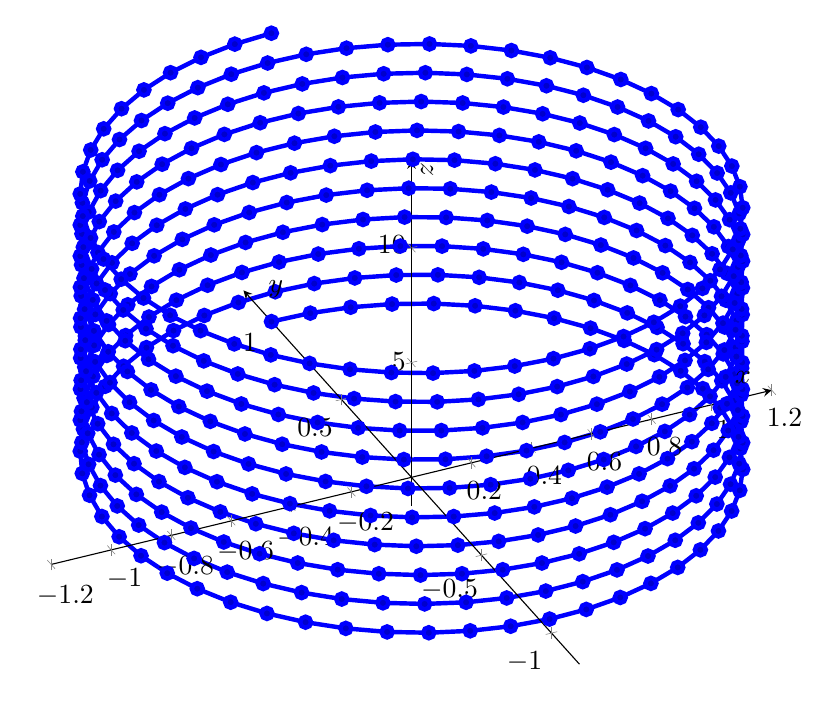
\begin{tikzpicture}
    \begin{axis}[
    axis lines=center,axis on top,
    colormap name=whitered,
    width=15cm,
    view={335}{50},
    enlargelimits=false,
    domain=-1:1,
    y domain=-1:1,
    samples=500, 
    xlabel=$x$,
    ylabel=$y$,
    zlabel={$z$},
    zlabel style={rotate=-90}, % Rotate z-label for better visibility
    every axis plot/.append style={ultra thick},
    enlarge x limits={0.1}, % Adjusted enlarge limits
    enlarge y limits={0.1}, % Adjusted enlarge limits
    enlarge z limits={0.1}% Adjusted enlarge limits % Increase plot thickness
    ]
        \addplot3+[domain=0:4*pi,samples y=0]
            ({sin(deg(5*x))},
             {cos(deg(5*x))},
             {x});
    \end{axis}
\end{tikzpicture}
